\section{Element objects - ELE}

In this section, the details of the implementation of the element 
objects are described. The relationship of element objects is shown 
in Fig. \ref{fig:ele_objects}. For the simulation of each process in 
a coupled problem or each single problem, only an instance of  mesh 
object (ELE-MSH) and an instance of finite element object are 
required. Geometric element object (ELE-GEO) manufacture the 
foundation of this concept (section \ref{sec:ele_geo}). Meshes 
(ELE-MSH) are formed based from geometric element entities (section 
\ref{sec:ele_msh}). Finite element object (ELE-FEM) basically 
compute the finite element matrices for different PDE types and 
geometric element types automatically  using the corresponding shape 
functions (section \ref{sec:ele_fem}).  ELE-PCS object assemble the 
equation systems for the problem type, i.e. THM coupled ELE-PCS 
object problems for porous media (section \ref{sec:ele_pcs}). 
\rev{To this purpose, objects  ELE-PCS and ELE-FEM and have a 
pointer member pointing to each other. When an instance of ELE-PCS 
object for a process in a coupled problem or a single problem is 
constructed, an instance of ELE-FEM object is created accordingly. 
During the construction of the instance of ELE-FEM object, the 
degree of freedom of the problem is initialized by the type the 
ELE-PCS instance, i.e. the specific problem. This means only one 
instance of ELE-PCS and one instance of ELE-FEM  have to been 
created for each process in a coupled problems or for each single 
problem. Moreover, ELE-FEM has a pointer member pointing to 
interpolation function. This member is initialized by the messages 
from the instance of ELE-PCS and each instance of ELE-GEO for each 
finite element during the local assembly. Such initialization 
guarantees that interpolation function and its derivatives are set 
properly for each geometric element for a process or a problem. 

\begin{figure}[!htb]
\centering
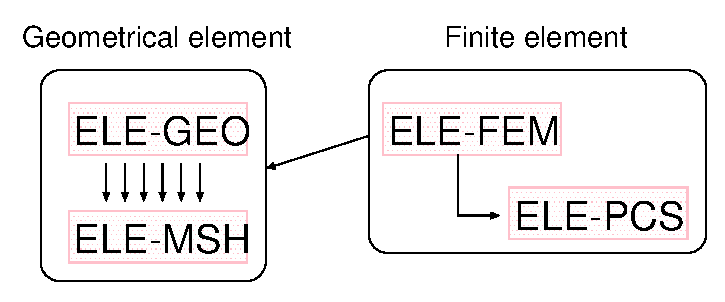
\includegraphics[scale=0.8]{figures/ele_relation.eps}
\caption{Relationship of element objects} 
\label{fig:ele_objects}
\end{figure}

In general, messages of the type of a process a problem and the type 
element determines the pointers to the corresponding interpolation 
function and its derivatives of an instance of ELE-FEM.   An 
instance of ELE-FEM has a pointer to  ELE-GEO as a member too. When 
local assembly comes to an element, or an instance of ELE-GEO, the 
ELE-FEM instance have the ELE-GEO pointer point to the element and 
initialized its numerical methods such as interpolation, Guass 
integration accordingly. This is very helpful for the finite element 
analysis of consolidation in porous media, in which, the Talyor-Hood 
finite element spaces, i.e. linear interpolation for flow process 
and quadratic interpolation for deformation process, is required for 
stability reason\cite{LeSch:98}. In default, the order of 
interpolation of each element is linear and the nodes of an element 
are its geometrical vertices.  If the high order interpolation is 
required by a process or a problem, additional nodes are created for 
each instance of ELE-FEM during the construction of the mesh.} The 
idea of this concept is, that specific process-related information 
are introduced as late as possible to keep the software concept as 
flexible as possible.

\subsection{Geometric element object -- ELE-GEO}
\label{sec:ele_geo}

As described in section \ref{sec:ovl}, the first step of finite
element analysis is the domain discretization. As a result we
obtain element meshes. Hereafter, we refer to a mesh element as
the geometric element object \texttt{ELE-GEO}. The intrinsic
properties of a geometric element object are: nodes, edges, faces, volume and neighbors (Fig. \ref{fig:elem}). Neighbor relationships connect
geometric element objects within a mesh and, therefore, represent
topological properties.

\begin{figure}[H]
\centering
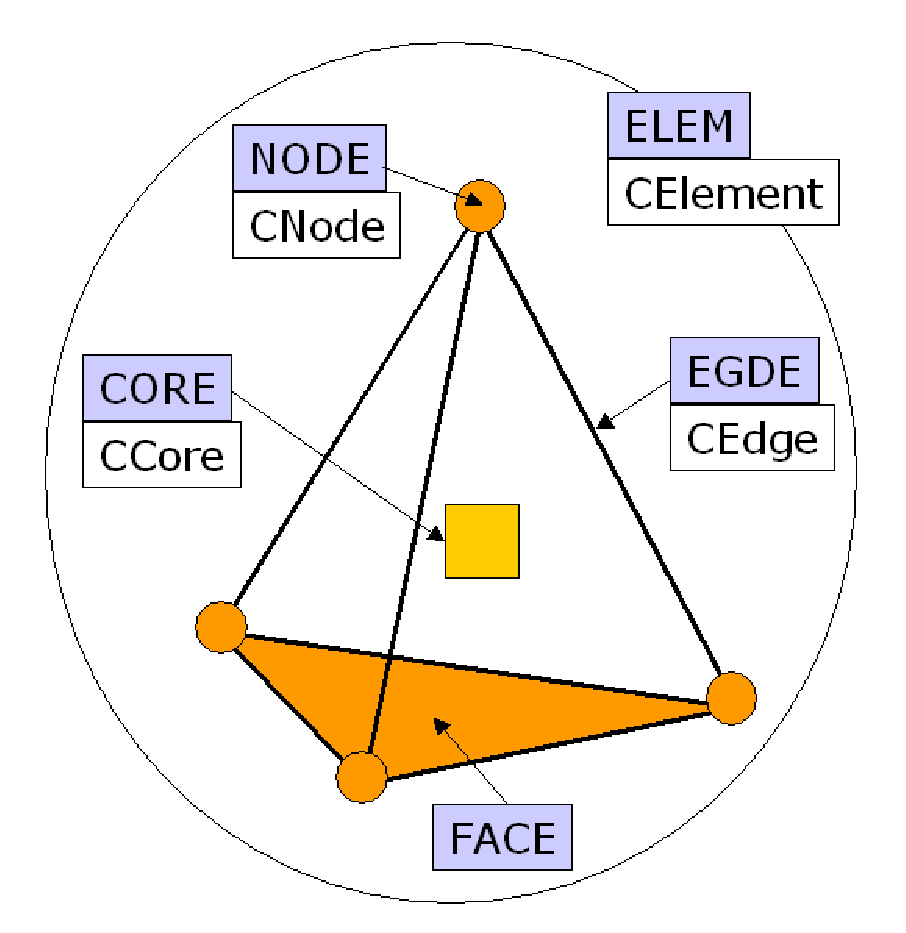
\includegraphics[scale=0.4]{figures/elem.eps}
\caption{Mesh element}
\label{fig:elem}
\end{figure}

%\begin{figure}[H]
%\centering
%\includegraphics[scale=0.7]{figure/gelement}
%\caption{Geometric element properties}
%\label{fig:gele}
%\end{figure}

We design the following element property classes to encapsulate
all geometric and topological element information.

\begin{itemize}
  \item \texttt{CCore} for \texttt{CORE} object,
  \item \texttt{CNode} for \texttt{NODE} object,
  \item \texttt{CEdge} for \texttt{EDGE} object,
  \item \texttt{CElem} for \texttt{ELEM} object.
\end{itemize}

Faces and neighbors belong to \texttt{ELEM} object. Indeed, edges
could be also assigned to the \texttt{ELEM} object. However, we
consider an edge as an individual entity for two reasons. First,
some numerical methods, such as mixed finite elements, require edges
as a basic geometric property as nodes for the Galerkin FEM. Second,
edges are frequently used as basic properties \rev{in automatic
generation}. As \texttt{NODE}, \texttt{EDGE} and \texttt{ELEM}
objects share common data and methods, we abstract these into the
\texttt{CCore} class as a base class.

\begin{figure}[H]
\centering
\shadowbox{
\begin{minipage}{0.9\textwidth}
{
\ttfamily \raggedright \small
\texttt{class\ CCore\\
\{\\
\ \ \ \textbf{protected}: // Properties\\
\ \ \ \ \ \ \textbf{long}\ index; // global element index\\
\ \ \ \ \ \ \textbf{char}\ position; // position indicator\\
%\ \ \ \ \ \ \textsl{//\ Status\ in\ usage}\\
\ \ \ \ \ \ \textbf{bool}\ status; //\ status\ in\ usage \\
%\ \ \ \ \ \ \textsl{//\ High\ order}\\
\ \ \ \ \ \ \textbf{int}\ order; // order of interpolation\\
\ \ \ \textbf{public}: // Methods\\
\ \ \ \ \ \ \textsl{//\ Set\ members}\\
\ \ \ \ \ \ \textbf{void}\ SetIndex(\textbf{const}\ \textbf{long}\ index)\ \{index\ =\ index;\}\\
\ \ \ \ \ \ \textbf{void}\ SetPosition(\textbf{const}\ \textbf{char}\ BC\underline\ type)\ \{boundary\ =\ BC\underline\ type;\}\\
\ \ \ \ \ \ \textbf{void}\ SetStatus(\textbf{const}\ \textbf{bool}\ status)\ \{status\ =\ status;\}\\
\ \ \ \ \ \ \textbf{void}\ SetOrder(\textbf{const}\ \textbf{int}\ order)\ \{order\ =\ order;\}\\
\ \ \ \ \ \ \textsl{//\ Get\ members}\\
\ \ \ \ \ \ \textbf{long}\ GetIndex()\ \textbf{const}\ \{\textbf{return}\ index;\}\ \\
\ \ \ \ \ \ \textbf{char}\ GetPosition()\ \textbf{const}\ \{\textbf{return}\ position;\}\ \\
\ \ \ \ \ \ \textbf{bool}\ GetStatus()\ \textbf{const}\ \{\textbf{return}\ status;\}\\
\ \ \ \ \ \ \textbf{int}\  GetOrder()\ \textbf{const}\ \{\textbf{return}\ order;\}\\
\ \ \ \ \ \ \textsl{//\ Construction}\\
\ \ \ \ \ \ CCore(\textbf{const}\ \textbf{int}\ id); // constructor\\
\ \ \ \ \ \ \textbf{virtual}\ \ \textasciitilde CCore(); // destructor\\
\ \ \ \ \ \ \textsl{//\ Operators}\\
\ \ \ \ \ \ \textbf{virtual}\ \textbf{void}\ \textbf{operator}\ =\ (\textbf{const}\ CCore\ \&\ g)\ \{\}\\
\ \ \ \ \ \ \textbf{virtual}\ \textbf{bool}\ \textbf{operator}\ ==\ (\textbf{const}\ CCore\ \&\ g)\ \{\textbf{return}\ \textbf{false};\}\\
\ \ \ \ \ \ \textsl{//\ Output}\\
\ \ \ \ \ \ \textbf{virtual}\ \textbf{void}\ output(ostream\&\ os=cout)\ \textbf{const}\ \{\};\\
\};\\
}
}
\normalfont\normalsize

\end{minipage}
}
\caption{\texttt{CCore} implementation for basic geometric element properties and methods}
\label{fig:core}
\end{figure}

\vfill

\newpage
%----------------------------------------------------------------------
\subsubsection{Core object - \texttt{CORE} - geometric element base class}
\label{sec:core}

Common data of a geometric element are: global element index;
position indicator within the whole domain, which indicates whether
the geometric element is inside the domain or on the domain surface;
%with specific boundary condition type;
status flag, which indicates whether this element is marked for
some usage. Assign $=$ as well as identity operators $==$ are
virtually defined. The C++ implementation of the \texttt{CCore} base
class is given in Fig. \ref{fig:coree}.

\begin{figure}[H]
\centering
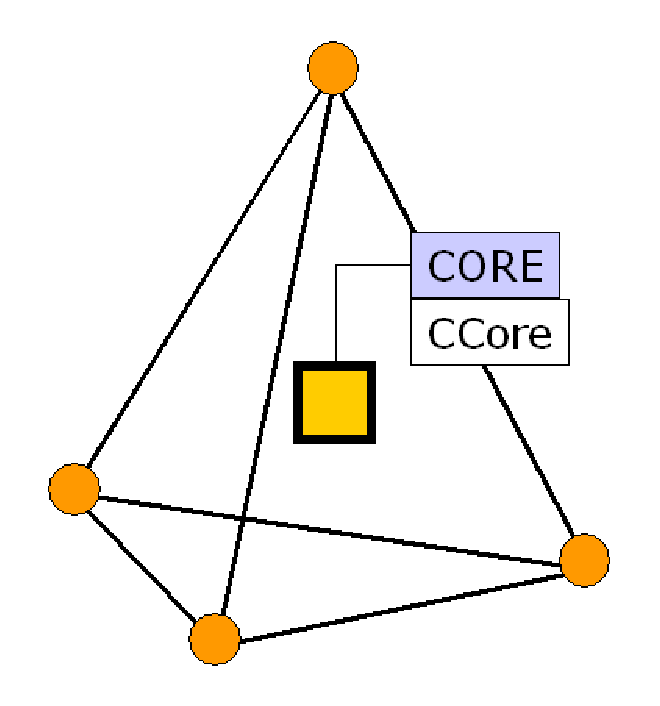
\includegraphics[scale=0.4]{figures/core.eps}
\caption{Core of mesh element} \label{fig:coree}
\end{figure}

\rev{Member \mbox{\texttt{char position}} is used to determine the
location of the geometrical entity within a domain, e.g. it is
inside the domain or on the boundary of the domain.}
%%\input{code/core}

Classes \texttt{CNode}, \texttt{CEdge} and \texttt{CElem} are
directly derived from the base class \texttt{CCore}. Assign $=$ as
well as the identity operator $==$ are overloaded in these
objects. With such overloading operators, passing data of an class
instance, \texttt{A}, to another class instance, \texttt{B}, can
be simply realized with the instruction
\mbox{\texttt{A}=\texttt{B}}. Whether two instances are identical
can be checked by the instruction
\mbox{\texttt{if}(\texttt{A}==\texttt{B})}.

\begin{figure}[H]
\centering
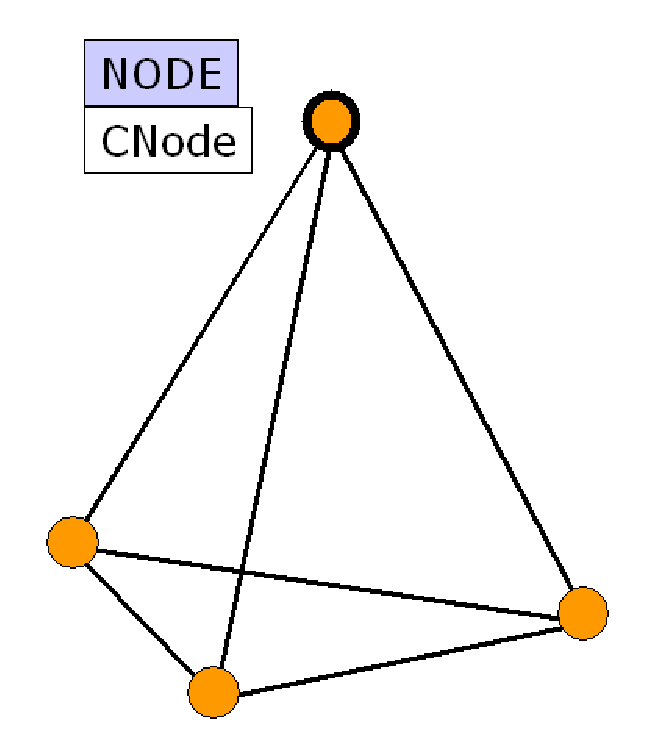
\includegraphics[scale=0.4]{figures/node.eps}
\caption{Node of element object} \label{fig:node1}
\end{figure}

%----------------------------------------------------------------------
\subsubsection{Node object - \texttt{NODE}}
\label{sec:node}

The node object (\texttt{NODE}) is derived from the \texttt{CCore}
class. In addition, the \texttt{CNode} class provides the
geometrical position of an element in real space, i.e. the coordinates
of element nodes (Fig. \ref{fig:node1}).

\begin{figure}[H]
\centering
\shadowbox{
\begin{minipage}{0.95\textwidth}
{\sffamily \raggedright
\footnotesize \texttt{class\ CNode:\textbf{public}\ CCore\\
\{\\
\ \ \ \textbf{private}: // Members\\
\ \ \ \ \ \ \textbf{double}\ coordinate[3];\\
\ \ \ \ \ \ Vector$<${}\textbf{long}$>${} ConnectedElements;\ \ \ \\
\ \ \ \ \ \ \rev{Vector$<${}\textbf{long}$>${} ConnectedNodes;}\ \ \ \\
\ \ \ \textbf{public}:\\
\ \ \ \ \ \ \textsl{//\ Construction}\\
\ \ \ \ \ \ Node(\textbf{const}\ \textbf{int}\ Index,\ \textbf{const}\ \textbf{double}\ x,\ \\
\ \ \ \ \ \ \ \ \ \ \ \textbf{const}\ \textbf{double}\ y,\ \textbf{const}\ \textbf{double}\ z=0.0);\\
\ \ \ \ \ \ Node()\ \{\}\\
\ \ \ \ \ \ \textasciitilde Node()\ \{ConnectedElements.resize(0); ConnectedNodes.resize(0);\}\\
\ \ \ \ \ \ \textsl{//\ Operators}\\
\ \ \ \ \ \ \textbf{void}\ \textbf{operator}\ =\ (\textbf{const}\ Node\&\ n);\\
\ \ \ \ \ \ \textbf{bool}\ \textbf{operator}\ ==\ (\textbf{const}\ Node\ \&\ n);\\
\ \ \ \ \ \ \textsl{//\ Set members}\\
\ \ \ \ \ \ \textbf{void}\ SetX(\textbf{const}\ \textbf{double}\ argX)\ \{\ coordinate[0]\ =\ argX;\}\\
\ \ \ \ \ \ \textbf{void}\ SetY(\textbf{const}\ \textbf{double}\ argY)\ \{\ coordinate[1]\ =\ argY;\}\\
\ \ \ \ \ \ \textbf{void}\ SetZ(\textbf{const}\ \textbf{double}\ argZ)\ \{\ coordinate[2]\ =\ argZ;\}\\
\ \ \ \ \ \ \textbf{void}\ SetCoordinates(\textbf{const}\ \textbf{double}$\ast$\ argCoord);\ \\
\ \ \ \ \ \ \textsl{//\ Get members}\\
\ \ \ \ \ \ \textbf{double}\ GetX()\ \textbf{const}\ \{\textbf{return}\ coordinate[0];\}\\
\ \ \ \ \ \ \textbf{double}\ GetY()\ \textbf{const}\ \{\textbf{return}\ coordinate[1];\}\\
\ \ \ \ \ \ \textbf{double}\ GetZ()\ \textbf{const}\ \{\textbf{return}\ coordinate[2];\}\\
%\ \ \ \ \ \ \textbf{void}\ Coordinates(\textbf{double}\ $\ast$xyz)\ \textbf{const}\\
%\ \ \ \ \ \ \{\ \ \textbf{for}(\textbf{int}\ i=0;\ i$<${}3;\ i++)\ \ xyz[i]\ =\ Coordinate[i];\}\ \\
\ \ \ \ \ \ \textbf{int}\ GetNumberOfConnectedElements()\ \textbf{const}\ \{\textbf{return}\ ConnectedElements.size();\ \}\ \ \ \ \ \\
\ \ \ \ \ \ \rev{\textbf{int}\ GetNumberOfConnectedNodes()\ \textbf{const}\ \{\textbf{return}\ ConnectedNodes.size();}\ \}\ \ \ \ \ \\
\ \ \ \ \ \ \textsl{//\ Output}\\
\ \ \ \ \ \ \textbf{void}\ Write(ostream\&\ os=cout)\ \textbf{const};\\
\ \ \ \textbf{private}: // Class relations\\
\ \ \ \ \ \ \textbf{friend}\ \textbf{class}\ CEdge;\\
\ \ \ \ \ \ \textbf{friend}\ \textbf{class}\ CElem;\\
\};\\
}
 }
\normalfont\normalsize

\end{minipage}
}
\caption{\texttt{CNode} implementation}
\label{fig:node}
\end{figure}

Mesh elements having this node in common are determined immediately
after mesh data is generated. Elements sharing this node are stored
in vector \texttt{ConnectedElements}. This node-element relationship
is very important information of the mesh topology. It is required
e.g. for extrapolation of Gauss point values to node values or for
projecting element properties to nodes. Using the
\texttt{ConnectedElements} vector, the calculation of mesh topology
can be enormously accelerated. \rev{For extrapolation of gauss point
values to nodes, we only need to know the size of the vector, i.e.
how many element connected to the nodes. Since extrapolation takes
place in element-wise, node values are accumulated from the
contribution of its connected elements, we have to average the
accumulated node value by dividing it with the number of connected
elements after extrapolation is finished. Member vector
\texttt{ConnectedNodes} stores indices of all nodes of connected
elements and it used together with the degree of freedom of the
preocess/problem to store indices of all nodes of connected elements
and it can be used together with the degree of freedom of the
preocess/problem to create the sparse matrix of the system
equations.to create the sparse matrix of the system equations. The
memory of \texttt{ConnectedNodes} is released as soon as the sparse
matrix is created.} Classes \texttt{CEdge} and \texttt{CElem} are
set as friend classes of \texttt{CNode} so that they can access to
\texttt{CNode} private members directly. The C++ implementation of
\texttt{class CNode} is given in Fig. \ref{fig:node}.

Instances of \texttt{NODE} object are stored in a global vector: \\
\texttt{vector<CNode*>node\_vector}.

%----------------------------------------------------------------------
\subsubsection{Edge object - \texttt{EDGE}}
\label{sec:edge}

The edge object (\texttt{EDGE}) is derived from the \texttt{CCore}
class. Edges are used to build up the frame of a geometric element
object (Fig. \ref{fig:gedge}). It is sufficient to use two nodes to
form a geometric edge. However, for higher order finite elements,
more points are required along an edge. Therefore, we use a vector
of \texttt{CNode} pointers as class member for edge nodes (see Fig.
\ref{fig:gedge}). In case of quadratic finite elements, the first
two nodes are element corner nodes and the last one is the middle
point of this edge.

\begin{figure}[H]
\centering
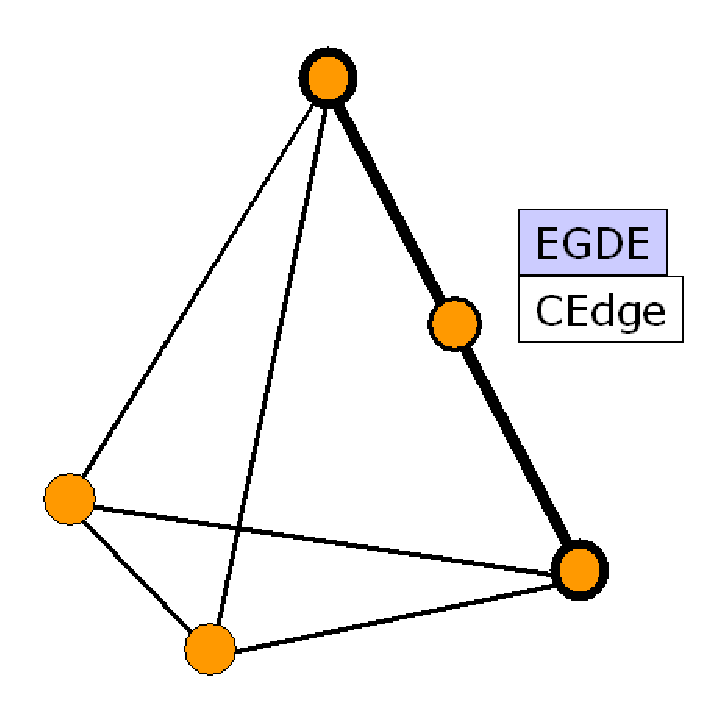
\includegraphics[scale=0.4]{figures/edge_new.eps}
\caption{Edge of mesh element} \label{fig:gedge}
\end{figure}

The C++ implementation of the \texttt{CEdge} class is given in
Fig. \ref{fig:edge}.

\texttt{Vector} is a "clone" of the standard C++ vector template,
as \texttt{template Vector\-<class V> class V} with less memory consuming but sufficient
and efficient functionality of vector algebraic calculation.

For node based finite elements (i.e. linear
interpolation), edges are only used to the compute topological mesh
structure \rev{and to process Dirichlet  boundary conditions and
source terms. For instance, if a Dirichlet  boundary condition of a
PDE is assigned by a polyline, edges of elements on the polyline
will be found and the Gauss integration will be performed on these
edges to produce node values of nodes of these edges}. They are not
needed to be stored for the later computations anymore. On the other
hand, mixed finite elements or higher order finite elements require
edges through all computations. In this case we save all edges of a
mesh in a standard C++ vector: \texttt{vector<CEdge*>egde\_vector}.

\begin{figure}[H]
\centering
\shadowbox{
\begin{minipage}{0.95\textwidth}
{
\sffamily \raggedright \scriptsize
\texttt{class\ CEdge:\textbf{public}\ CCore\\
\{\\
\ \ \ \textbf{private}: // Members\\
\ \ \ \ \ \ vec$<${}CNode$\ast>${}\ nodes\underline\ of\underline\ edges;\\
\ \ \ \textbf{public}: // Member functions\\
\ \ \ \ \ \ \textsl{//\ Construction}\\
\ \ \ \ \ \ Edge(\textbf{const}\ \textbf{int}\ Index,\ \textbf{bool}\ quadr=\textbf{false});\\
\ \ \ \ \ \ \textasciitilde Edge();\ \\
\ \ \ \ \ \ \textsl{//\ Operators}\\
\ \ \ \ \ \ \textbf{void}\ \textbf{operator}\ =\ (CEdge\&\ edg);\\
\ \ \ \ \ \ \textbf{bool}\ \textbf{operator}\ ==\ (CEdge\&\ edg);\\
\ \ \ \ \ \ \textsl{//\ Member access}\\
\ \ \ \ \ \ \textbf{void}\ SetNodes(\ vec$<${}CNode$\ast>${}\&\ Nodes)\\
\ \ \ \ \ \ \{\ \textbf{for}(\textbf{int}\ i=0;\ i$<${}(\textbf{int})Nodes.Size();\ i++)\ \ Nodes[i]\ =\ nodes\underline\ of\underline\ edges[i];\ \}\\
\ \ \ \ \ \ \textbf{void}\ SetNodes(\ vec$<${}CNode$\ast>${}\&\ Nodes)\ \textbf{const}\ \{\ Nodes\ =\ nodes\underline\ of\underline\ edges;\}\\
\ \ \ \ \ \ \textsl{//\ Output}\\
\ \ \ \ \ \ \textbf{void}\ Write(ostream\&\ osm=cout)\ \textbf{const};\\
\ \ \ \textbf{private}: // Class relations\\
\ \ \ \ \ \ Vector$<${}CNode$\ast>${}\ \ nodes\underline\ of\underline\ edges;\\
\ \ \ \ \ \ \textbf{friend}\ \textbf{class}\ CElem;\\
\};\\
}
 }
\normalfont\normalsize

\end{minipage}
}
\caption{\texttt{CEdge} implementation}
\label{fig:edge}
\end{figure}

%
\begin{figure}[H]
\centering
\shadowbox{
\begin{minipage}{0.9\textwidth}
{
\sffamily \raggedright \scriptsize
\texttt{class\ CElement:\textbf{public}\ CCore\\
\{\\
\ \ \ \textbf{private}:\ \textsl{//\ Members}\\
\ \ \ \ \ \ \textsl{//\ ID}\\
\ \ \ \ \ \ CElem$\ast$\ owner;\\
\ \ \ \ \ \ \textbf{int}\ ele\underline\ type;\ \ \textsl{//\ Element\ type}\\
\ \ \ \ \ \ \textsl{//\ Geometrical properties}\\
\ \ \ \ \ \ \textbf{int}\ dim;\ \ \ \ \ \ \ \textsl{//\ dimension\ of\ element}\\
\ \ \ \ \ \ \textbf{double}\ volume;\ \textsl{// element volume}\\
\ \ \ \ \ \ \textsl{//\ Topological properties}\\
\ \ \ \ \ \ \textbf{int}\ nnodes;\ \ \ \ \textsl{//\ number\ of element corner nodes}\\
\ \ \ \ \ \ \textbf{int}\ nnodesHQ;\ \ \textsl{//\ number of element nodes for quadratic interpolation}\\
\ \ \ \ \ \ Vector$<${}CNode$\ast>${}\ \ nodes;\\
\ \ \ \ \ \ \textbf{int}\ nedges;\ \ \ \ \textsl{//\ number\ of\ edges}\\
\ \ \ \ \ \ Vector$<${}CEdge$\ast>${}\ \ edges;\\
\ \ \ \ \ \ \textbf{int}\ nfaces;\ \ \ \ \textsl{//\ number\ of\ faces}\\
\ \ \ \ \ \ \textsl{//\ Mesh topology}\\
\ \ \ \ \ \ \textbf{int}\ sub\_domain;\\
\ \ \ \ \ \ Vector$<${}CElem$\ast>${}\ \ neighbors;\\
\ \ \ \ \ \ Vector$<${}CElem$\ast>${}\ \ sons;\\
%%\ \ \ \ \ \ \textsl{//\ ???}\\%%
\ \ \ \ \ \ Vector$<${}\textbf{long}$>${}\ \ \ nodes\underline\ index;\\
\}\\
}
 }
\normalfont\normalsize

\end{minipage}
}
\caption{\texttt{CElem} implementation}
\label{fig:gelee}
\end{figure}
%

%----------------------------------------------------------------------
\subsubsection{Element object - \texttt{ELEM}}
\label{sec:elem}

The element object (\texttt{ELEM}) is also derived from the
\texttt{CCore} class. \texttt{ELEM} represents an individual
element of a mesh. Node and edge objects are employed to construct
the element object. An abstract mesh element object is designed
for different geometric element types, i.e. lines, triangles,
quadrilaterals, tetrahedra, triangle based prisms, hexahedra
(Table \ref{tab:elem}, Fig. \ref{fig:ele_types}). These geometric
element types are defined by an ID, i.e, integer number represent
element type.
The C++ implementation of \texttt{class CElem} is given in Fig.
\ref{fig:gelee}.

Basic members of the element object are identification,
geometrical as well as topological properties and mesh
relationships.
%
Element ID (index) is inherited from the \texttt{CORE} object.
Dimension and volume are basic geometric members. Depending on the
geometric type of an element (\texttt{ele\_type}), the following
 geomatrical and topological properties are specified:

\begin{table}[H]
\caption{Basic topology information of an geometrical element}
\begin{center}
% use packages: array
\begin{tabular}{lccccc}
\hline
Geometric type  & \texttt{ele\_type}&\texttt{nnodes}& \texttt{nnodesHQ}& \texttt{nfaces} & \texttt{nedges}\\
\hline
Line &1& 2&3& &\\
Quadrilateral&2&4&9& 4&4\\
Hexehedron&3& 8&20& 6&12\\
Triangle&4&  3&6& 3&3\\
Tetrahedron & 5& 4&10& 4&6\\
Prism &6  & 6&15& 5&9\\
\hline
\label{tab:elem}
\end{tabular}
\end{center}
\end{table}


Element nodes and edges are kept in the following two member vectors

\texttt{$\quad$Vector$<${}CNode$\ast>${}\ nodes;} 

and

\texttt{$\quad$Vector$<${}CEdge$\ast>${}\ edges;}

%The element configuration is conducted based on the geometric
%element type with member function {\texttt{CElem::Config(long
%element\_index}}. By this the corresponding \texttt{ELEM} members
%are created and initialized (Table \ref{tab:elem}).

\begin{figure}[htb!]
\centering
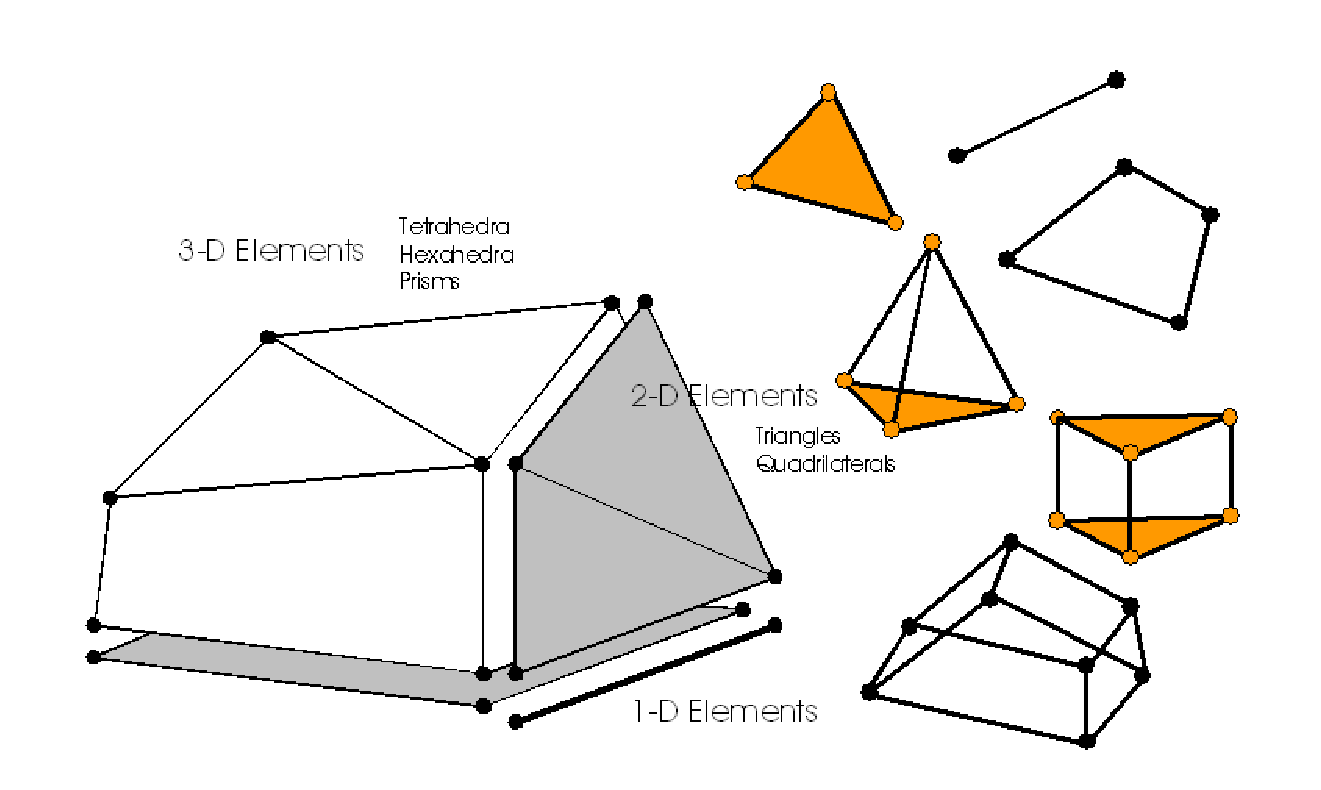
\includegraphics[scale=0.55]{figures/elements.eps}
\caption{Geometric elements types} \label{fig:ele_types}
\end{figure}

\subsection{Finite element object -- ELE-FEM}
\label{sec:ele_fem}

In this section we present the design of the finite element object, 
i.e. properties and methods, which are required to conduct the finite 
element analysis. In particular, we discuss the implementation of 
steps 2 and 3 described in  Table 
\ref{tab:alg1}, i.e., local element assembly and global assembly of system 
equation.

%In the present study, we consider the node based finite element
%and numerical integration of local finite element calculations.

%One of the advantages of object oriented programming is data
%encapsulation. In the encapsulation sense, all data, i.e.
%information, of an object are arranged to live in a scope only.
%This guarantees the safety of data within the running of
%corresponding programme as much as possible.

According to the principles of object-oriented programming, we
encapsulate common data and functionalities of finite elements into 
a base class. There are two general tasks of the finite element 
object. First, local finite element calculations and, second, 
contributions of the element to the global equation system.
%
Afterwards, we derive specific finite element objects for
different problem types (i.e. PDE types) in the framework of THM
porous media mechanics (see Fig. \ref{fig:ele_concept}).

\emph{Finite element base class:}
%
Local element calculations require the selection of specific
interpolation functions as well as their derivatives at
integration points corresponding to different element types.
Therefore, element interpolation functions are regarded as basic
items of the finite element object.
%
%We consider element interpolation functions of all kinds of
%geometric element types as global functions that are visible
%through the whole code.
%
These interpolation functions have two arguments: first, values of
shape functions or the derivative of shape functions; second,
reference points, e.g. Gauss points.
%The values of this first argument is calculated with coordinates
%of a reference point coordinates passed in through the second
%argument.
Therefore, for each kind of geometric element type, we have four
functions associated with element interpolation as

%%\small
\begin{verbatim}
  void ShapeFunctionXXXX(double*,double*);
  void ShapeFunctionHQXXXX(double*,double*);
  void GradShapeFunctionXXXX(double*,double*);
  void GradShapeFunctionHQXXXX(double*,double*);
\end{verbatim}
%%\normalsize

where \texttt{XXXX} is specifying the different geometric element
types. \texttt{ShapeFunction\-XXXX} provides linear interpolation
functions $\Sh_1$, whereas \texttt{ShapeFunctionHQXXXX} gives
quadratic interpolation functions $\Sh_2$, mentioned in section
\ref{sec:fem}. \texttt{GradShape\-FunctionXXXX} and
\texttt{GradShapeFunctionHQXXXX} offer the derivatives of the
corresponding interpolation functions $\Sh_1$ and $\Sh_2$,
respectively. Interpolation functions for all kinds of element types are declared as global functions. 
The function pointer 
\texttt{void (*VoidFuncDXCDX) (double*,double*)}
is defined to point to the addresses of the global interpolation 
functions. 
 The C++ implementation of the finite element base class \texttt{CElement} is 
given in Fig. \ref{fig:fem_root}.

\begin{figure}[htb!]
\centering
\shadowbox{
\begin{minipage}{\textwidth}
\scriptsize
\begin{verbatim}
class CFiniteElement {
  protected: // Member data
    CElem* m_ele_geo; // Instance of geometric element
    int order; //Order of shape functions
    int n_gauss_points; // Number of Gauss points
    int n_gauss; // Number of sample points for Gauss integration
    mutable double unit[4]; // Local element coordinates
    double* Jacobian; // Jacobian matrix
    double* invJacobian; // Inverse Jacobian matrix
    double* shape_fct; // Linear shape function values at Gauss points
    double* shape_fct_HQ; // Quadratic shape function values at Gauss points
    double* d_shape_fct; // Linear shape function derivative values at Gauss points
    double* d_shape_fct_HQ; // Quadratic shape function derivative values at
                            // Gauss points
  public: // Member functions
    CFiniteElement(const int order=1);
    virtual ~CFiniteElement();
    virtual void Config(CElem* m_ele_geo);
    virtual void ConfigNumerics(const int type);
    double GetGaussData(const int gp,int& gp_r,int& gp_s,int& gp_t)
    virtual void ComputeShapeFct(const int order);
    virtual void ComputeGradShapeFct(const int order);
    virtual double ComputeJacobian(const int order);
    virtual void RealCoordinates(double*xyz);
    virtual void RefCoordinates(double*xyz);
    virtual void LocalAssembly();
    virtual void FaceIntegration();
  protected: // Member functions
    VoidFuncDXCDX ShapeFunction; // Prototype for linear shape functions
    VoidFuncDXCDX ShapeFunctionHQ; // Prototype for quadratic shape functions
    VoidFuncDXCDX GradShapeFunction; // Prototype for linear shape function derivatives
    VoidFuncDXCDX GradShapeFunctionHQ; // Prototype for quadratic shape 
                                       // function derivatives
}
\end{verbatim}
\normalfont\normalsize

\end{minipage}
}
\caption{Finite element base class}
\label{fig:fem_root}
\end{figure}

Member variable, \texttt{m\_ele\_geo}, is a pointer to the
corresponding geometric element object \texttt{CElem}, which links
the finite element object to geometry. When the local assembly
takes place for an element, the instance of this element is
obtained by finite element object with its member function,
\texttt{void Config(CElem\* m\_ele\_geo)}. With this, the finite
element object has all geometrical and topological properties such as geometric type,
coordinate nodes, neighbors for local element calculation.

%Element configuration is based on the geometric element type. The
%C++ implementation of the \texttt{Config} function is presented in
%Fig. \ref{fig:fem_num}.
%
%\input{code/fem_num}

Different weak forms arise from the different governing equations
of flow problem, heat transport problem and mechanical problem
(eqn. (\ref{eq:wkmass}), (\ref{eq:wkhTmass}) and
(\ref{eq:wkstress})). This requires different element level
computations for the specific problem. Since root finite element
object provides the basic numerical functionality, we can use 
this object directly for the benefit of the polymorphism mechanism
of object oriented programming.


%=========================================================================
\subsection{Process related finite element objects -- ELE-PCS}
\label{sec:ele_pcs}

Only at this stage (last part of element object concept) we
introduce process-related data. The element object
\texttt{CFiniteElementPCS} should work for all processes: fluid
flow, heat transport, deformation and reaction processes
regardless of PDE type and type of unknown field functions (scalar
or vector quantities).

The finite element object ELE-PCS has two tasks: First, calculation 
of element matrices, which are formed by shape functions 
($\Sh_1,\nabla\Sh_1$) and process-specific material properties 
(\texttt{MAT} objects) (Step 2 in Table \ref{tab:alg1}). Second, 
provide local element contributions to the global equation system: 
$A_{ij} x_i = b_j$, where $i,j$ are global node indices (Step 3 in 
Table \ref{tab:alg1}).

The C++ implementation of the process-related finite element
object ELE-PCS is given in Fig. \ref{fig:fem_one}.

\begin{itemize}
%.........................................................................
 \item ELE-FEM relation:
Process related instances are derived from the finite element base
class \texttt{CFiniteElement}. Therefore, they inherit all
necessary geometric and topological data from ELE-GEO, ELE-FEM,
and ELE-MSH objects.
%.........................................................................
 \item PCS relation:
Process related finite element objects need a reference to the
related PCS instance, which is conducted by the ELE-PCS class
constructor.
%.........................................................................
 \item MAT relations:
References to all \texttt{MAT} objects, i.e.
\texttt{CFluidProperties* m\_mfp}, \texttt{CSolidProper\-ties*
m\_msp} and \texttt{CMediumProperties* m\_mmp}, are used to get
the required material parameters of the specified
process(\texttt{CProcess* m\_pcs}). Member function
\texttt{SetMaterial()} prepares the references to process-specific
material properties to accelerate later computations. This insures
that the ELE-FEM objects works properly for all THM processes,
i.e. fluid flow, heat transport and deformation.
%.........................................................................
 \item Local assembly - Element matrices:
Based on geometric and finite element base data (ELE-FEM relation)
and the references to material data (PCS-MAT relation) the
process-specific element matrices can be calculated now
(\texttt{CalcXXXXMatrix()}). Member functions are used to
calculate the material coefficients in the Gauss integration
points (\texttt{CalcXXXXMatrixCoefficients()}). They are defined
as \texttt{inline} types to improve the computation efficiency.
Local element matrices and vectors are stored in the corresponding
symmetric/unsymmetric matrix and vector constructs.
%.........................................................................
 \item Global assembly - Equation system:
The global assembly is conducted by the \texttt{Assemble()}
function. It updates the individual element contributions in the
equation system, i.e. global left-hand-side (LHS) matrix
($A_{ij}$) and global right-hand-side (RHS) vector ($b_j$). To
this purpose the assembly functions needs the relations between
local element node and global mesh node numbers, which is provided
by the ELE-MSH topology (section \ref{sec:ele_msh}).
\texttt{Assemble()} functions are available for different PDE
types. How the \texttt{Assemble()} is implemented for a parabolic
PDE is shown in Fig. \ref{fig:fem_asm}.
\end{itemize}

\begin{figure}[htb!]
\centering
\shadowbox{
\begin{minipage}{\textwidth}
\footnotesize
\begin{verbatim}
class CFiniteElementPCS::public CFiniteElement {
  private: // Member data
    // PCS relation
    CProcess* m_pcs;
    // MAT relations
    CFluidProperties* m_mfp;
    CSolidProperties* m_mfp;
    CMediumProperties* m_mmp;
    // Element matrices
    SymMatrix* MassMatrix;
    SymMatrix* LaplaceMatrix;
    SymMatrix* PressureCouplingMatrix;
    Matrix*    AdvectionMatrix;
    Matrix*    StrainMatrix;
    Matrix*    StrainCouplingMatrix;
    ...
    Matrix*    LHSMatrix;
    Vec*       RHSVector;
  public:  // Member functions
    // Construction
    CFiniteElementPCS(CProcess* m_pcs);
    ~CFiniteElementPCS();
    // MAT functions
    void SetMaterial();
    inline void CalcMassMatrixCoefficient();
    inline void CalcAdvectionMatrixCoefficient();
    inline void CalcLaplaceMatrixCoefficient();
    inline void CalcStrainMatrixCoefficient();
    inline void CalcStrainCouplingMatrixCoefficient();
    inline void CalcPressureCouplingMatrixCoefficient();
    // Element matrices
    inline double InterpolateGPValues(double*); // Interpolation at Gauss points
    void SetMemory();
    void CalcMassMatrix();
    void CalcLumpedMassMatrix();
    void CalcAdvectionMatrix();
    void CalcLaplaceMatrix();
    void CalcStrainMatrix();
    void CalcStrainCouplingMatrix();
    void CalcPressureCouplingMatrix();
    void CalcGravityVector();
    void LocalAssembly(); // LHS element contribution
    ...
    // Element contribution to global equation system
    void GlobalAssembly(); // LHS matrix contribution
}
\end{verbatim}
\normalfont\normalsize

\end{minipage}
}
\caption{Process related finite element class}
\label{fig:fem_one}
\end{figure}


\begin{figure}[H]
\centering
\shadowbox{
\begin{minipage}{0.7\textwidth}
\small
\begin{verbatim}
void CFiniteElementPCS::AssembleParabolicPDEType()
{
  // MAT relations
  SetMaterial();
  // Calculation and assembly of element matrices
  CalcMassMatrix();
  CalcLaplaceMatrix();
  CalcStrainCouplingMatrix();
  // Calculation and assembly of RHS vector
  CalcRHSVector();
}
\end{verbatim}
\normalfont\normalsize

\end{minipage}
}
\caption{Linear element assemble function}
\label{fig:fem_asm}
\end{figure}

%-------------------------------------------------------------------------
%\subsubsection{Finite element objects for vector field functions}

%Deformation process is governed by the Navier's equation. The
%local element matrices like tangential matrix (\ref{eq:Tang}) has
%different expression in addition to those arise from the Laplace
%type equations. Moreover, the non-linear analysis of such problems
%involving complex local calculation. To this purpose, a
%corresponding finite element object is derived from root finite
%element object.
%The C++ implementation of the quadratic FEOs for
%deformation problems is given in Fig. \ref{fig:fem_dm}.

%\input{code/fem_dm.tex}

%In addition to the standard finite element object defined in section
%\ref{sec:finone}, this class needs a reference to solid material
%properties.

%The solid phase material object (\texttt{MSP}) provides the
%constitutive stress-strain relationships for linear as well as
%nonlinear behavior. While fluid material object allows deformation
%finite element object incorporate the coupling calculation.

%Element stiffness matrix, eqn. (\ref{eq:Tang}), pressure coupling
%matrix, eqn. (\ref{eq:CMatrix}), and RHS vector are calculated by
%member function \texttt{LocalAssembly} and assembled to the global
%equation system by member function \texttt{GlobalAssembly}.
%Modified local assemble functions are required for enhanced strain
%element calculations.

\subsection{Element-Mesh relations -- ELE-MSH}
\label{sec:ele_msh}

From Fig. \ref{fig:ele_objects} it can be seen, that element-mesh
relations have multiple functions in the element concept, e.g.
\begin{itemize}
 \item ELE-GEO relation: mesh topology, neighbor relationships of
 geometric elements, element connectivity, incorporation of of boundary
 conditions,
 \item ELE-FEM relation: coordinate transformation between local
 element and global coordinates,
 \item ELE-PCS relation: local element nodes and node index in the
 global equation system, material domains.
\end{itemize}

\subsubsection{ELE-GEO relation}

Apart from the individual/intrinsic element properties, the
\texttt{ELEM} object contains information about mesh topology,
i.e. how this element is emplaced in the element mesh. For
instance, the (\texttt{sub\_domain}) index indicates the part of
the domain to which this element belongs. This number is used e.g.
to distinguish elements in different areas of the domain with
different material properties. Neighbor relationships of geometric
elements are important topological properties of an element mesh.
Neighbors of an element are all those elements adjacent to the
faces of the element. Since the definition of \texttt{ELEM} object
provides necessary functionality of different geometric element
types, we use pointers to \texttt{ELEM} object itself to recode
neighbors as

\texttt{Vector$<${}CElem$\ast>${}\ neighbors;}

\begin{figure}[H]
 \centering
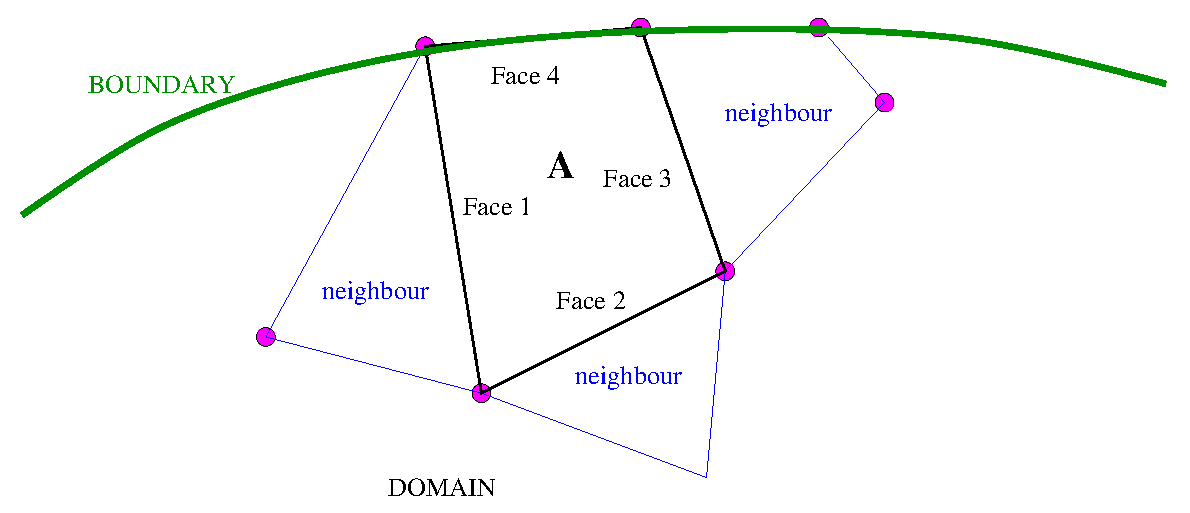
\includegraphics[scale=0.6]{figures/neighbor.eps}
\caption{Definition of element neighbors} \label{fig:gnei}
\end{figure}

As an example Fig. \ref{fig:gnei} illustrates the arrangement of
neighbor relationships in 2D space, in which quadrilateral
element A has three neighbor elements adjacent to its faces (i.e.
edges in 2D) 1, 2 and 3. Neighbors 1 and 2 are triangle elements,
while neighbor 3 is a quadrilateral element. Face 4 is on the
domain boundary, which is not shared by any other element. Vector
member, \texttt{neighbors}, is initialized with size of 4 and
assigned during mesh construction. The first three entries are
assigned with pointers to neighbors 1, 2 and 3. The last entry of
the vector is filled with a pointer to a surface (Face 4), which
is an instance of \texttt{ELEM} object configured for a line
element. The boundary type \texttt{position} of this instance is
set as 'B'. The coding of the element neighboring process is given
below:

\small
\begin{center}
\begin{verbatim}
neighbors[0] = (CElem*) Neighbour1;
neighbors[1] = (CElem*) Neighbour2;
neighbors[2] = (CElem*) Neighbour3;
neighbors[3] = (CElem*) Face4;
Face4->position = 'B'; // on domain boundary
Face4->owner = this; // this element
\end{verbatim}
\end{center}
\normalsize

The above neighbor vector is a member of element,
i.e., ELEM, object.

\subsubsection{ELE-FEM relation}

The ELE-FEM association concerns coordinate transformation between
local element and global coordinates. Depending on the geometric
and numerical type of a finite element, related shape functions
and their derivatives are available (section \ref{sec:ele_fem}).
%%This is particularly important for hybrid meshes (Fig.
%%\ref{ffig:gnei}). 
Jacobian calculations are another typical ELE-FEM methods.

\subsubsection{ELE-PCS relation}

Subdomain properties of element are used to describe heterogeneity, 
i.e. local variation of material properties for different problems. 
Element neighbor relationships are essential data for constructing 
the mesh and determine the propagation orientation of 
discontinuities in failure analysis (section \ref{sec:apl_m}). 
Moreover, the proposed element concept allows the assignment of 
different processes (PCS objects) and meshes (MSH objects). 
%%This is an important feature for upscaling procedures \cite{Kol:2005b}.

